
\documentclass[5pt]{article}

\usepackage{sectsty}
\usepackage{graphicx}
\usepackage{lipsum} % for generating dummy text
\usepackage[margin=1in]{geometry}
\usepackage{setspace}
\usepackage{array}
\usepackage{cellspace}
\usepackage{tabularx}
\usepackage[table]{xcolor}
\usepackage{tabularray}
\usepackage{pgfplots}


\usepackage{hyperref}
\usepackage{scrextend}
\graphicspath{ {../assets} }


% Margins
\topmargin=-0.45in
\evensidemargin=0in
\oddsidemargin=0in
\textwidth=6.5in
\textheight=9.0in
\headsep=0.25in

\setlength{\parindent}{0pt}

\title{Piano di Qualifica}
\author{Jackpot Coding}
\renewcommand*\contentsname{Indice}
\date{\today}

%STARTOF THE DOCUMENT
\begin{document}
	
	%-------------------------
	
	% Reduce top margin only on the first page
	\newgeometry{top=0.5in}
	
	%UNIPD LOGO
	\vspace{8pt}
	
\includegraphics[scale=0.2]{UNIPDFull.png}
	%END UNIPD LOGO
	
	\vspace{30pt}
	
	%COURSE INFO
	\begin{minipage}[t]{0.48\textwidth}
		%COURSE TITLE
		\begin{flushleft}
			Informatica\\
			\vspace{5pt}
			\textbf{\LARGE Ingegneria del Software}\\
			Anno Accademico: 2023/2024
		\end{flushleft}
		%END COURSE TITLE
	\end{minipage}
	%END COURSE INFO
	
	
	\vspace{5px}
	
	
	%BLACK LINE
	\rule{\textwidth}{5pt}
	
	%JACKPOT CODING INFO
	\begin{minipage}[t]{0.50\textwidth}
		%LOGO JACKPOT CODING
		\begin{flushleft}
			\hspace{10pt}
			
\includegraphics[scale=0.65]{jackpot-logo.png} 
		\end{flushleft}
	\end{minipage}
	\hspace{-60pt} % This adds horizontal space between the minipages
	\begin{flushright}
		\begin{minipage}[t]{0.50\textwidth}
			%INFO JACKPOT CODING
			\begin{flushright}
				Gruppo: {\Large Jackpot Coding}\\
				Email: \href{mailto:jackpotcoding@gmail.com}{jackpotcoding@gmail.com}
			\end{flushright}
		\end{minipage}
	\end{flushright}
	%END JACKPOT CODING INFO
	
	\vspace{24pt}
	
	%TITLE
	\begin{center}
		\textbf{\LARGE PIANO DI QUALIFICA}
	\end{center}
	%END TITLE
	
	\vspace{13pt}
	
	\begin{flushleft}
		\begin{spacing}{1.5}
			REDATTORI: G. Moretto, R. Simionato, M. Gobbo\\%INSERT HERE THE NAMES
			VERIFICATORI: \\
			\vspace{7pt}
			DESTINATARI: Prof. T. Vardanega, Prof. R. Cardin\\%INSERT HERE THE NAMES
		\end{spacing}
	\end{flushleft}
	
	\begin{flushright}
		\begin{spacing}{1}
			USO: ESTERNO\\
			VERSIONE: 0.1.9\\
		\end{spacing}
	\end{flushright}
	
	
	% Restore original margins from the second page onwards
	\restoregeometry
	
	\pagebreak
	
	\textbf{\Large Registro delle modifiche}
	\begin{table}[ht]
		\centerline{%
			\begin{tabular}{|c|c|c|c|c|}
				\hline
				v.0.1.9 & 21/03/2024 & R. Simionato & - & Aggiunti struttura grafici MPC-CV, MPC-AC e MPC-ETC \\
				\hline
				v.0.1.8 & 20/03/2024 & R. Simionato & - & \shortstack{Aggiunti grafici MPC-RSI e MPD-CO\\Aggiunte sottosezioni per altri grafici} \\
				\hline
				v.0.1.7 & 19/03/2024 & G. Moretto & - & Aggiunta grafico MPD-I \\
				\hline
				v.0.1.6 & 19/03/2024 & G. Moretto & - & Aggiunta grafici MPC-SV e MPC-NCR \\
				\hline
				v.0.1.5 & 18/03/2024 & G. Moretto & - & Verifica termini di glossario \\
				\hline
				v.0.1.4 & 18/03/2024 & R. Simionato & G. Moretto & Stesura sezioni 2.1.2, 2.2, 2.3 \\
				\hline
				v.0.1.3 & 17/03/2024 & M. Gobbo & G. Moretto & Aggiunta Sezione 3-Qualità di Prodotto \\
				\hline
				v.0.1.2 & 17/03/2024 & R. Simionato & G. Moretto & Aggiunta struttura Sezione 3-Qualità di Prodotto \\
				\hline
				v.0.1.1 & 16/03/2024 & R. Simionato & G. Moretto & \shortstack{Prima stesura sezione Qualità di Processo\\e inserimento tabelle} \\
				\hline
				v.0.1.0 & 16/03/2024 & - & R. Simionato & Verifica Documento \\
				\hline
				v.0.0.3 & 14/03/2024 & G. Moretto & R. Simionato & Aggiunta sezione Valutazione attività di verifica \\
				\hline
				v.0.0.2 & 13/02/2024 & G. Moretto & R. Simionato  &  Aggiunte descrizioni test\\
				\hline
				v.0.0.1 & 03/02/2024 & G. Moretto & R. Simionato  & Creata struttura del documento \\
				\hline
			\end{tabular}%
		}
		\label{tab:conference}
	\end{table}
	
	
	
	\pagebreak
	\tableofcontents
	\pagebreak
	
	% Elenco Figure
	% Elenco Tabelle
	
	\section{Introduzione}
	
	\subsection{Premessa}
	Questo documento viene modificato durante la durata del progetto ed i suoi contenuti verranno aggiornati in base alle pratiche adottate dal gruppo.
	
	\subsection{Scopo del documento}
	Lo scopo di questo documento è quello di raccogliere:
	\begin{itemize}
		\item Obiettivi della qualità di Prodotto;
		\item Obiettivi della qualità di Processo;
		\item Metodi per la misurazione di questi tramite metriche;
		\item Definizione dei test da effettuare;
		\item Cruscotto\textsuperscript{G} per la visione dello stato del raggiungimento degli obiettivi;
	\end{itemize}
	
	\subsection{Scopo del prodotto}
	Il capitolato\textsuperscript{G} proposto dall'azienda Zucchetti manifesta l'esigenza di avere un prodotto \textit{Software}\textsuperscript{G} per la creazione di \textit{prompt}\textsuperscript{G} da fornire ad un modello\textsuperscript{G} \textit{LLM}\textsuperscript{G} per la creazione di \textit{query} SQL\textsuperscript{G} per l'interrogazione di \textit{database}\textsuperscript{G} con struttura nota.
	
	
	\section{Qualità di Processo}
	Per garantire la qualità del prodotto bisogna essere in grado di assicurarsi che i processi raggiungano gli obiettivi di qualità richiesti. In questa sezione vengono definite le metriche utilizzate per valutare i processi e per migliorarli secondo il Ciclo PDCA (\textit{Plan-Do-Check-Act}). Questo metodo permette un miglioramento continuo nell’applicazione dei processi e l’utilizzo delle risorse a disposizione tramite la pianificazione, seguita dalla messa in atto, verifica utilizzando le metriche a disposizione e infine miglioramento dei processi.
	
	\subsection{Processi primari}
	\subsubsection{Fornitura}
	Processo basato sulla scelta delle risorse e procedure da utilizzare per lo sviluppo del progetto.
	\begin{longtblr}
		{
			colspec={|Q[0.15\linewidth]|Q[0.25\linewidth]|Q[0.25\linewidth]|Q[0.25\linewidth]|},
			columns={halign=c},
			row{1}={halign=c},
			row{odd} = {gray!20},
			row{1}={teal!50},
			%caption=Tabella 1
		}
		\hline
		\textbf{Metrica} & \textbf{Descrizione} & \textbf{Valore Accettabile} & \textbf{Valore Ottimale} \\
		%codice & descrizione & valAcc & valOtt \\
		\hline
		MPC-EAC & \textit{Estimated At Completion} & Errore del $\pm$5\% rispetto al preventivo & Corrispondente al preventivo \\
		\hline
		MPC-ETC & \textit{Estimated To Completion} & $\geq$ 0\% & $\leq$ EAC \\
		\hline
		MPC-EV & \textit{Earned Value} & $\geq$ 0 & $\leq$ EAC \\
		\hline
		MPC-PV & \textit{ Planned Value} & $\geq$ 0 & $\leq$ Costo totale del preventivo \\
		\hline
		MPC-AC & \textit{Actual Cost} & $\geq$ 0 & $\leq$ EAC \\
		\hline
		MPC-CV & \textit{Cost Variance} & $\geq$ -5\% & $\geq$ 0\% \\
		\hline
		MPC-SV & \textit{Schedule Variance} & $\geq$ -10\% & $\geq$ 0\% \\
		\hline
		MPC-BV & \textit{Budget Variance} & $\pm$10\% & $\leq$ 0\% \\
		\hline
	\end{longtblr}
	
	\subsubsection{Sviluppo}
	Processo basato sulla scelta delle attività e dei compiti necessari per la realizzazione del prodotto \textit{software}\textsuperscript{G}.
	\begin{longtblr}
		{
			colspec={|Q[0.15\linewidth]|Q[0.25\linewidth]|Q[0.25\linewidth]|Q[0.25\linewidth]|},
			columns={halign=c},
			row{1}={halign=c},
			row{odd} = {gray!20},
			row{1}={teal!50},
			%caption=Tabella 1
		}
		\hline
		\textbf{Metrica} & \textbf{Descrizione} & \textbf{Valore Accettabile} & \textbf{Valore Ottimale} \\
		%codice & descrizione & valAcc & valOtt \\
		\hline
		MPC-RSI & \textit{Requirements Stability Index} & $\geq$ 80\% & 100\% \\
		\hline
		MPC-SOR & \textit{Satisfied Obligatory Requirements} & 100\% & 100\% \\
		\hline
	\end{longtblr}
	
	\subsection{Processi di supporto}
	\subsubsection{Gestione della qualità}
	Processo necessario a garantire gli obiettivi di qualità del prodotto e dei servizi offerti.
	\begin{longtblr}
		{
			colspec={|Q[0.15\linewidth]|Q[0.25\linewidth]|Q[0.25\linewidth]|Q[0.25\linewidth]|},
			columns={halign=c},
			row{1}={halign=c},
			row{odd} = {gray!20},
			row{1}={teal!50},
			%caption=Tabella 1
		}
		\hline
		\textbf{Metrica} & \textbf{Descrizione} & \textbf{Valore Accettabile} & \textbf{Valore Ottimale} \\
		%codice & descrizione & valAcc & valOtt \\
		\hline
		MPC-QMS &\textit{ Quality Metric Satisfied} & $\geq$ 90\% & 100\% \\
		\hline
	\end{longtblr}
	
	\subsubsection{Verifica}
	Processo che ha lo scopo di controllare lo sviluppo del \textit{software}\textsuperscript{G} dal lato della codifica.
	\begin{longtblr}
		{
			colspec={|Q[0.15\linewidth]|Q[0.25\linewidth]|Q[0.25\linewidth]|Q[0.25\linewidth]|},
			columns={halign=c},
			row{1}={halign=c},
			row{odd} = {gray!20},
			row{1}={teal!50},
			%caption=Tabella 1
		}
		\hline
		\textbf{Metrica} & \textbf{Descrizione} & \textbf{Valore Accettabile} & \textbf{Valore Ottimale} \\
		%codice & descrizione & valAcc & valOtt \\
		\hline
		MPC-CC & \textit{Code Coverage} & $\geq$ 70\% & $\geq$ 90\% \\
		\hline
		MPC-PTP & \textit{Passed Tests Percentage} & $\geq$ 90\% & 100\% \\
		\hline
	\end{longtblr}
	
	\subsection{Processi organizzativi}
	\subsubsection{Gestione organizzativa}
	Processo che controlla le modalità di coordinamento del gruppo.
	\begin{longtblr}
		{
			colspec={|Q[0.15\linewidth]|Q[0.25\linewidth]|Q[0.25\linewidth]|Q[0.25\linewidth]|},
			columns={halign=c},
			row{1}={halign=c},
			row{odd} = {gray!20},
			row{1}={teal!50},
			%caption=Tabella 1
		}
		\hline
		\textbf{Metrica} & \textbf{Descrizione} & \textbf{Valore Accettabile} & \textbf{Valore Ottimale} \\
		%codice & descrizione & valAcc & valOtt \\
		\hline
		MPC-NCR & \textit{Non-Calculated Risks} & $\leq$ 5 & 0 \\
		\hline
	\end{longtblr}
	
	
	\section{Qualità di Prodotto}
	Dopo aver individuato le caratteristiche necessarie ed utili per la gestione del ciclo di vita del \textit{software}\textsuperscript{G}, il gruppo \textit{Jackpot Coding} ha rivolto lo sguardo a quali potessero essere le caratteristiche fondamentali per la realizzazione di un prodotto di qualità.
	
	\subsection{Obiettivi}
	\textbf{Documenti}
	\begin{longtblr}
		{
			colspec={|Q[0.25\linewidth]|Q[0.50\linewidth]|Q[0.15\linewidth]|},
			columns={halign=c},
			row{1}={halign=c},
			row{odd} = {gray!20},
			row{1}={teal!50},
			%caption=Tabella 1
		}
		\hline
		\textbf{Obiettivo} & \textbf{Descrizione} & \textbf{Metrica} \\
		%codice & descrizione & valAcc \\
		\hline
		Comprensione & Il corretto redigere dei documenti è cruciale per la qualità del nostro prodotto. È fondamentale assicurarsi che siano comprensibili e privi di errori, sia a livello lessicale che grammaticale & MPD-IG MPD-CO \\
		\hline
	\end{longtblr}
	
	\textbf{\textit{Software}}
	\begin{longtblr}
		{
			colspec={|Q[0.25\linewidth]|Q[0.50\linewidth]|Q[0.15\linewidth]|},
			columns={halign=c},
			row{1}={halign=c},
			row{odd} = {gray!20},
			row{1}={teal!50},
			%caption=Tabella 1
		}
		\hline
		\textbf{Obiettivo} & \textbf{Descrizione} & \textbf{Metrica} \\
		%obiettivo & descrizione & metriche \\
		\hline
		Funzionalità & La capacità del prodotto \textit{software}\textsuperscript{G} di soddisfare 
		i requisiti\textsuperscript{G} trovati e descritti all’interno dell’Analisi dei Requisiti\textsuperscript{G}. & MPD-CR \\
		\hline
		Efficienza\textsuperscript{G} & Svolgere il lavoro in un tempo consono alla quantità 
		di risorse utilizzate & MPD-TM \\
		\hline
		Usabilità & Creazione di un \textit{software} che sia semplice ed 
		intuitivo da utilizzare e comprendere, alla portata di ogni utente\textsuperscript{G} & MPD-TA MPD-RO MPD-EU \\
		\hline
		Affidabilità & La tolleranza del prodotto \textit{software} agli errori 
		quando usato in date condizioni per un dato periodo. & MPD-FD \\
		\hline
		Manutenibilità & La capacità del \textit{software} ad essere incline a 
		modifiche, miglioramenti in corso d'opera & MPD-CC \\
		\hline
		Portabilità & La capacità del \textit{software} di poter essere utilizzato 
		senza problemi in altri browser\textsuperscript{G} oltre a quello di sviluppo & MPD-BS \\
		\hline
	\end{longtblr}
	
	
	\subsection{Metriche}
	\textbf{Documenti}
	\begin{longtblr}
		{
			colspec={|Q[0.15\linewidth]|Q[0.25\linewidth]|Q[0.25\linewidth]|Q[0.25\linewidth]|},
			columns={halign=c},
			row{1}={halign=c},
			row{odd} = {gray!20},
			row{1}={teal!50},
			%caption=Tabella 1
		}
		\hline
		\textbf{Metrica} & \textbf{Descrizione} & \textbf{Valore Accettabile} & \textbf{Valore Ottimale} \\
		%codice & descrizione & valAcc & valOtt \\
		\hline
		MPD-IG  & Indice \textit{Gulpease} - Misura la leggibilità del testo & 40/100 & 60/100\\
		\hline
		MPD-CO & Correttezza Ortografica - Numero di errori grammaticali o ortografici & 0 & 0\\
		\hline
	\end{longtblr}
	
	\textbf{\textit{software}}
	\begin{longtblr}
		{
			colspec={|Q[0.15\linewidth]|Q[0.25\linewidth]|Q[0.25\linewidth]|Q[0.25\linewidth]|},
			columns={halign=c},
			row{1}={halign=c},
			row{odd} = {gray!20},
			row{1}={teal!50},
			%caption=Tabella 1
		}
		\hline
		\textbf{Metrica} & \textbf{Descrizione} & \textbf{Valore Accettabile} & \textbf{Valore Ottimale} \\
		%codice & descrizione & valAcc & valOtt \\
		\hline
		MPD-CR & Copertura dei Requisiti\textsuperscript{G} & 100 \% & 100 \% \\
		\hline
		MPD-TM & Tempo di risposta Medio & ? & ? \\
		\hline
		MPD-TA & Tempo di Apprendimento & 10 min & 5 min \\
		\hline
		MPD-RO & Raggiunta dell’Obiettivo & 6 click & 4 click \\
		\hline
		MPD-EU & Errori Utente\textsuperscript{G} & 2 & 0 \\
		\hline
		MPD-FD &\textit{ Failure Density} & 100\% & 100\% \\
		\hline
		MPD-CC & Complessità del Codice & ? & ? \\
		\hline
		MPD-BS & \textit{Browser}\textsuperscript{G} Supportati & 75\% & 100\% \\
		\hline
	\end{longtblr}
	
	
	\section{Specifica dei Test}
	
	\subsection{Test di Unità}
	Vengono impiegati per la verifica di unità del \textit{software}\textsuperscript{G}. Come unità si intende una piccola parte del programma che funzioni in maniera autonoma.
	
	\subsection{Test di Integrazione}
	Vengono impiegati per la verifica delle interazioni fra le unità sopra descritte.
	
	\subsection{Test di Sistema}
	Vengono impiegati per verificare che l'esecuzione del sistema soddisfi i requisiti\textsuperscript{G} prestabiliti nel documento di Analisi dei Requisiti\textsuperscript{G}.
	
	\subsection{Test di Regressione}
	Vengono impiegati per accertarsi che correzioni o aggiunte effettuate sul specifiche unità non interferiscano sul funzionamento del programma.
	
	\subsection{Test di Accettazione}
	Detto anche collaudo, viene effettuato per verificare che i requisiti\textsubscript{G} utente siano soddisfatti. Questo test viene effettuato assieme al committente\textsubscript{G}.
	
	
	\section{Resoconto attività di verifica}
	
	\subsection{Fornitura}
	\subsubsection{MPC-CV (\textit{Cost Variance})}
	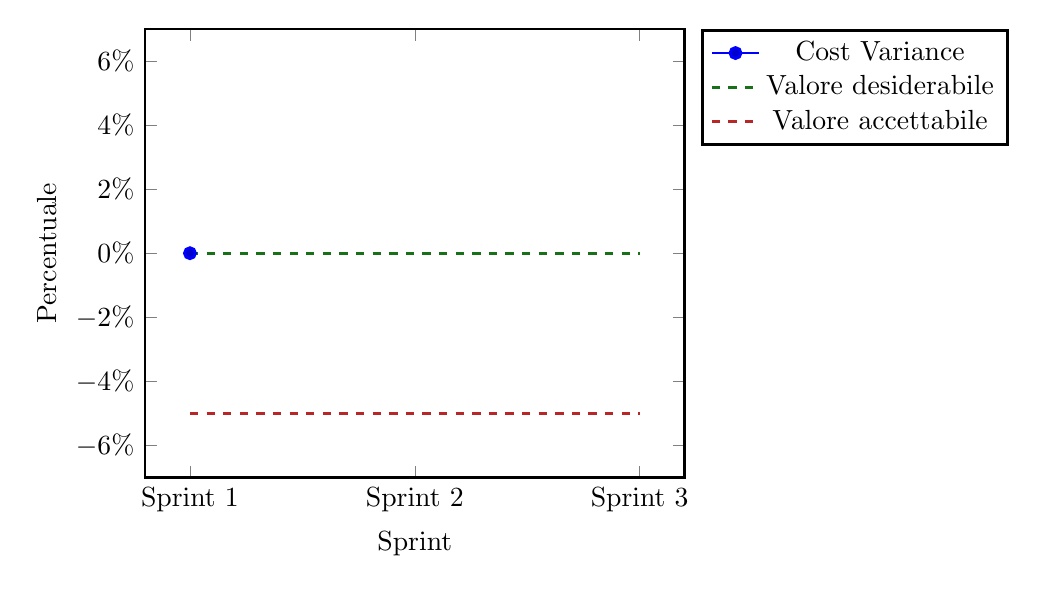
\begin{tikzpicture}
		\begin{axis}[
			xticklabels={Sprint 1, Sprint 2, Sprint 3},
			xtick={0,1,2},
			xlabel=Sprint,
			ytick={-6,-4,-2,0,2,4,6},
			ylabel=Percentuale,
			ymax=7,
			ymin=-7,
			line width=1.0,
			yticklabel={\pgfmathprintnumber{\tick}\%},
			legend style={ 
				legend pos =outer north east
			},
			legend columns=1
			]
			]
			\addplot+[sharp plot, blue] coordinates { (0,0) };
			\addlegendentry{Cost Variance}
			
			\addplot[mark=none, dashed, green4 ]  coordinates { (0,0) (2,0) };
			\addlegendentry{Valore desiderabile}
			
			\addplot[mark=none, dashed, red4]  coordinates { (0,-5) (2,-5) };
			\addlegendentry{Valore accettabile}
			
		\end{axis}
	\end{tikzpicture}
	
	\subsubsection{MPC-AC e MPC-ETC (\textit{Actual Cost} e \textit{Estimate To Completion})}
	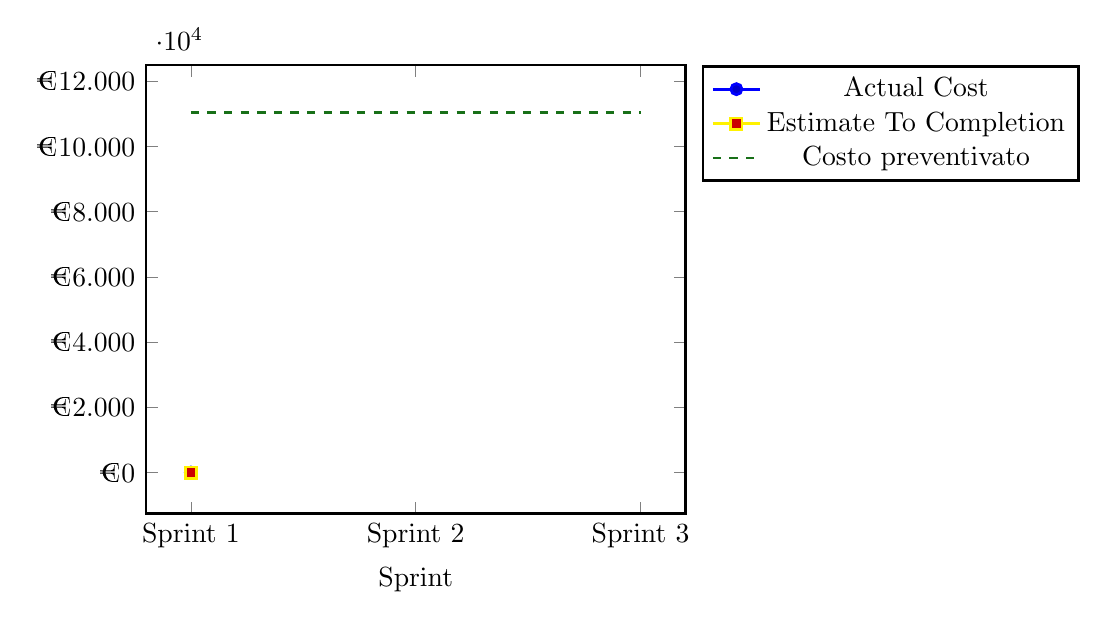
\begin{tikzpicture}
		\begin{axis}[
			xticklabels={Sprint 1, Sprint 2, Sprint 3},
			xtick={0,1,2},
			xlabel=Sprint,
			ytick={0,2000,...,12000},
			%ylabel=Costo,
			ymax=12500,
			%ymin=-7,
			line width=1.0,
			%yticklabel={\tick\texteuro},
			%y tick label style={xshift=-0.2em,log ticks with fixed point},
			yticklabels={\texteuro0, \texteuro2.000, \texteuro4.000, \texteuro6.000, \texteuro8.000, \texteuro10.000, \texteuro12.000},
			legend style={ 
				legend pos =outer north east
			},
			legend columns=1
			]
			]
			\addplot+[sharp plot, blue] coordinates { (0,0) };
			\addlegendentry{Actual Cost}
			
			\addplot+[sharp plot, yellow] coordinates { (0,0) };
			\addlegendentry{Estimate To Completion}
			
			\addplot[mark=none, dashed, green4 ]  coordinates { (0,11040) (2,11040) };
			\addlegendentry{Costo preventivato}
			
		\end{axis}
	\end{tikzpicture}
	
	\subsubsection{MPC-SV (\textit{Schedule Variance})}
	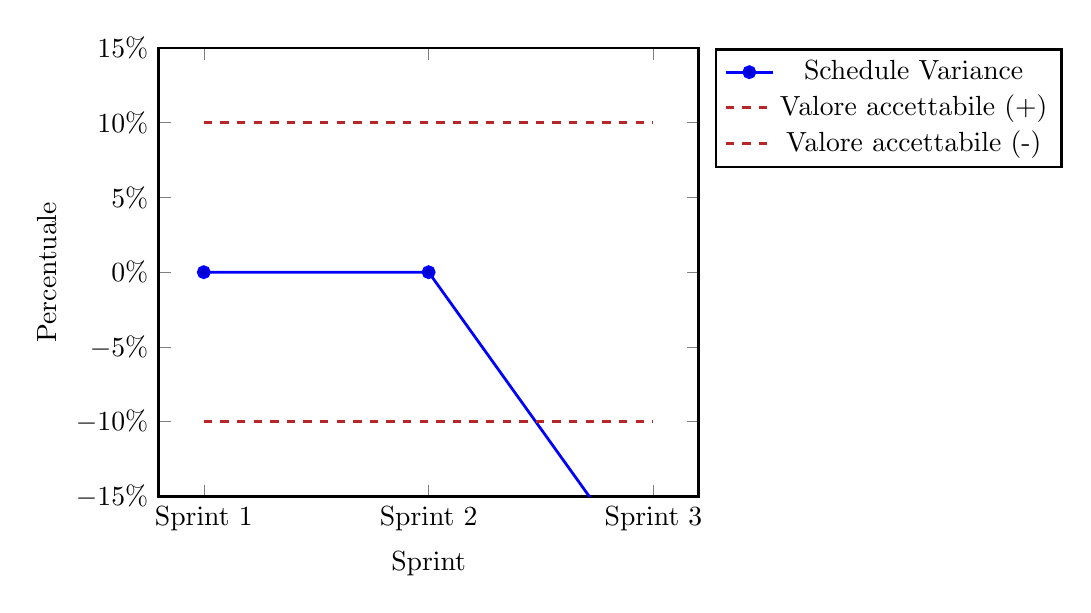
\begin{tikzpicture}
		\begin{axis}[
			xticklabels={Sprint 1, Sprint 2, Sprint 3},
			xtick={0,1,2},
			xlabel=Sprint,
			ytick={-15,-10,-5,0,5,10,15},
			ylabel=Percentuale,
			ymax=15,
			ymin=-15,
			line width=1.0,
			yticklabel={\pgfmathprintnumber{\tick}\%},
			legend style={ 
				legend pos =outer north east
			},
			legend columns=1
			]
			]
			\addplot+[sharp plot, blue] coordinates {(0,0) (1,0) (2,-21) };
			\addlegendentry{Schedule Variance}
			
			\addplot[mark=none, dashed, red4 ]  coordinates { (0,10) (2,10) };
			\addlegendentry{Valore accettabile (+)}
			
			\addplot[mark=none, dashed, red4]  coordinates { (0,-10) (2,-10) };
			\addlegendentry{Valore accettabile (-)}
			
		\end{axis}
	\end{tikzpicture}
	
	\subsection{Sviluppo}
	\subsubsection{MPC-RSI (\textit{Requirements Stability Index})}
	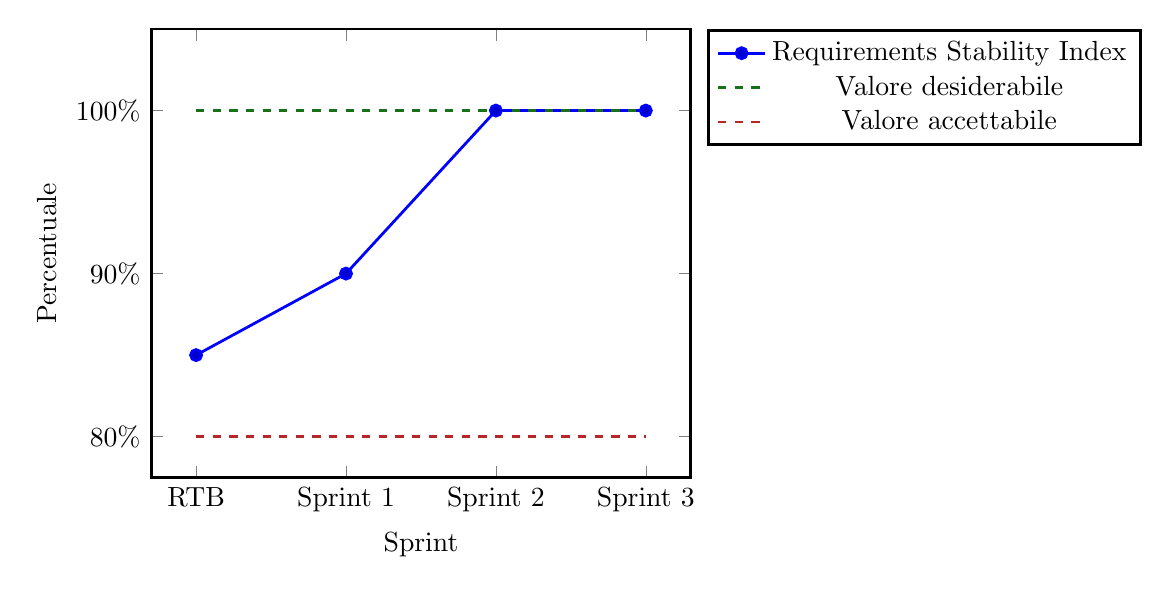
\begin{tikzpicture}
		\begin{axis}[
			xticklabels={RTB, Sprint 1, Sprint 2, Sprint 3},
			xtick={0,1,2,3},
			xlabel=Sprint,
			ytick={0,10,...,100},
			ylabel=Percentuale,
			%yticklabels={\pgfmathprintnumber{\tick}\%},
			yticklabel=\pgfmathprintnumber{\tick}\%,
			ymax=105,
			line width=1.0,
			legend style={ 
				legend pos =outer north east
			},
			legend columns=1
			]
			]
			\addplot+[sharp plot, blue] coordinates {(0,85) (1,90) (2,100) (3,100) };
			\addlegendentry{Requirements Stability Index}
			
			\addplot[mark=none, dashed, green4]  coordinates { (0,100) (3,100) };
			\addlegendentry{Valore desiderabile}
			
			\addplot[mark=none, dashed, red4 ]  coordinates { (0,80) (3,80) };
			\addlegendentry{Valore accettabile}
			
		\end{axis}
	\end{tikzpicture}
	
	\subsection{Gestione di qualità}
	
	\subsection{Verifica}
	
	\subsection{Processi organizzativi}
	
	% non-calculated risk
	\subsubsection{MPC-NCR (\textit{Non-Calculated Risks)}}
	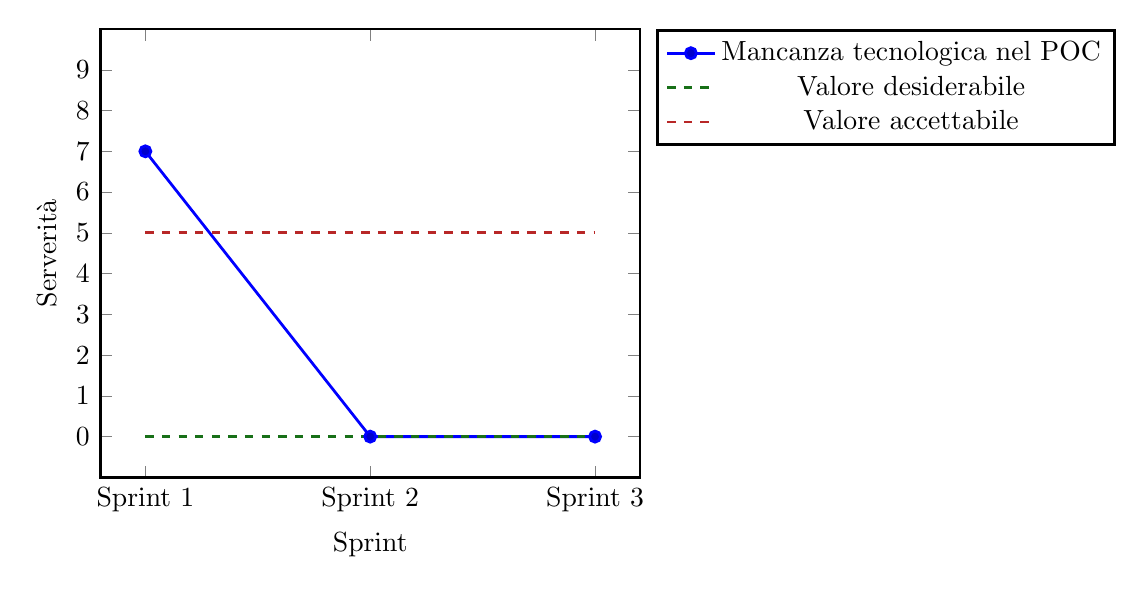
\begin{tikzpicture}
		\begin{axis}[
			xticklabels={Sprint 1, Sprint 2, Sprint 3},
			xtick={0,1,2},
			xlabel=Sprint,
			ytick={0,1,...,9},
			ylabel=Serverità,
			yticklabels={0,1,...,9},
			ymax=10,
			line width=1.0,
			legend style={ 
				legend pos =outer north east
			},
			legend columns=1
			]
			]
			\addplot+[sharp plot, blue] coordinates {(0,7) (1,0) (2,0) };
			\addlegendentry{Mancanza tecnologica nel POC}
			
			\addplot[mark=none, dashed, green4]  coordinates { (0,0) (2,0) };
			\addlegendentry{Valore desiderabile}
			
			\addplot[mark=none, dashed, red4 ]  coordinates { (0,5) (2,5) };
			\addlegendentry{Valore accettabile}
			
		\end{axis}
	\end{tikzpicture}
	
	\subsection{Gestione organizzativa}
	
	\subsection{Documenti}
	
	\subsubsection{MPD-IG (Indice Gulpease)}
	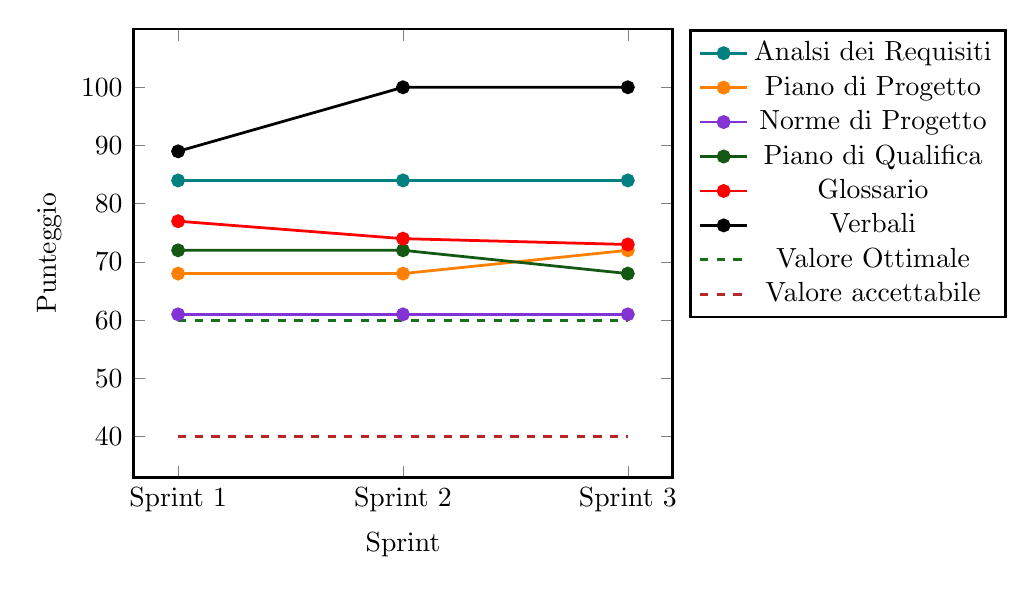
\begin{tikzpicture}
		\begin{axis}[
			xticklabels={Sprint 1, Sprint 2, Sprint 3},
			xtick={0,1,2},
			xlabel=Sprint,
			ytick={30,40,50,60,70,80,90,100},
			ylabel=Punteggio,
			ymax=110,
			line width=1.0,
			legend style={ 
				legend pos =outer north east
			},
			legend columns=1
			]
			]
			\addplot+[sharp plot, teal, mark=*, solid, mark options={fill=teal}] coordinates {(0,84) (1,84) (2,84)  };
			\addlegendentry{Analsi dei Requisiti}
			
			\addplot+[sharp plot, orange, solid, mark=*, mark color=orange, mark options={fill=orange}] coordinates {(0,68) (1,68) (2,72) };
			\addlegendentry{Piano di Progetto}
			
			\addplot+[sharp plot,violet4, solid, mark=*, mark options={fill=violet4}] coordinates {(0,61) (1,61) (2,61) };
			\addlegendentry{Norme di Progetto}
			
			\addplot+[sharp plot,green3, solid, mark=*, mark options={fill=green3}] coordinates {(0,72) (1,72) (2,68) };
			\addlegendentry{Piano di Qualifica}
			
			\addplot+[sharp plot, red, solid, mark=*, mark options={fill=red}] coordinates {(0,77) (1,74) (2,73)  };
			\addlegendentry{Glossario}			
			
			\addplot+[sharp plot, black, solid, mark=*, mark options={fill=black}] coordinates {(0,89) (1,100) (2,100)  };
			\addlegendentry{Verbali}			
			
			\addplot[mark=none, dashed, green4, mark=none]  coordinates { (0,60) (2,60) };
			\addlegendentry{Valore Ottimale}
			
			\addplot[mark=none, dashed, red4,mark=none]  coordinates { (0,40) (2,40) };
			\addlegendentry{Valore accettabile}
			
		\end{axis}
	\end{tikzpicture}
	
	\subsubsection{MPD-CO (Correttezza Ortografica)}
	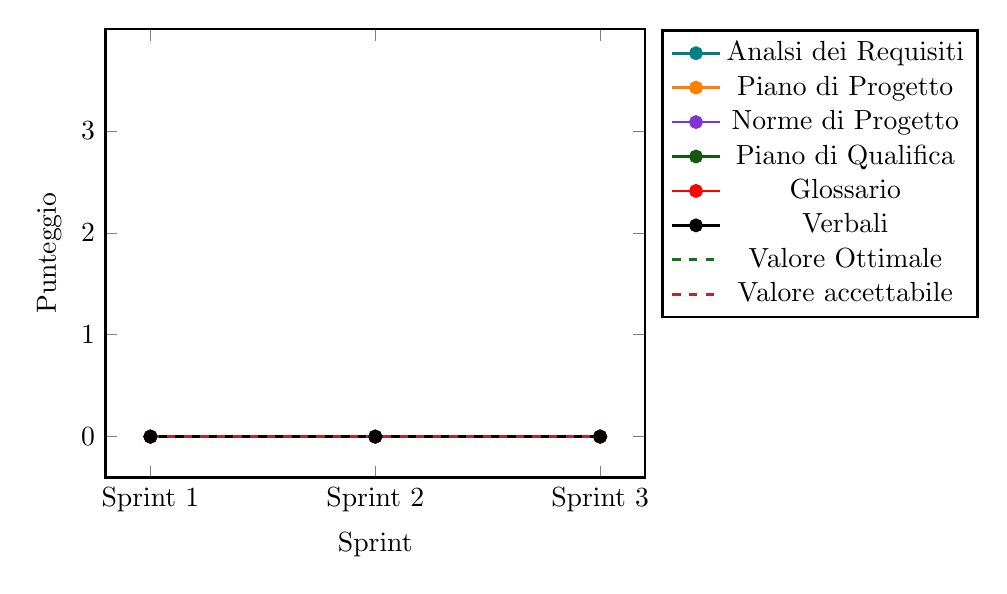
\begin{tikzpicture}
		\begin{axis}[
			xticklabels={Sprint 1, Sprint 2, Sprint 3},
			xtick={0,1,2},
			xlabel=Sprint,
			ytick={0,1,2,3},
			ylabel=Punteggio,
			ymax=4,
			line width=1.0,
			legend style={ 
				legend pos =outer north east
			},
			legend columns=1
			]
			]
			\addplot+[sharp plot, teal, mark=*, solid, mark options={fill=teal}] coordinates {(0,0) (1,0) (2,0)  };
			\addlegendentry{Analsi dei Requisiti}
			
			\addplot+[sharp plot, orange, solid, mark=*, mark color=orange, mark options={fill=orange}] coordinates {(0,0) (1,0) (2,0) };
			\addlegendentry{Piano di Progetto}
			
			\addplot+[sharp plot,violet4, solid, mark=*, mark options={fill=violet4}] coordinates {(0,0) (1,0) (2,0) };
			\addlegendentry{Norme di Progetto}
			
			\addplot+[sharp plot,green3, solid, mark=*, mark options={fill=green3}] coordinates {(0,0) (1,0) (2,0) };
			\addlegendentry{Piano di Qualifica}
			
			\addplot+[sharp plot, red, solid, mark=*, mark options={fill=red}] coordinates {(0,0) (1,0) (2,0)  };
			\addlegendentry{Glossario}			
			
			\addplot+[sharp plot, black, solid, mark=*, mark options={fill=black}] coordinates {(0,0) (1,0) (2,0)  };
			\addlegendentry{Verbali}			
			
			\addplot[mark=none, dashed, green4, mark=none]  coordinates { (0,0) (2,0) };
			\addlegendentry{Valore Ottimale}
			
			\addplot[mark=none, dashed, red4,mark=none]  coordinates { (0,0) (2,0) };
			\addlegendentry{Valore accettabile}
			
		\end{axis}
	\end{tikzpicture}
	
	
	
	\section{Valutazioni delle attività di verifica}
	In questa sezione si riportano le valutazioni sulle criticità incontrate nel corso dello svolgimento del progetto e le correzioni applicate ad esse.
	
	\subsection{Organizzazione}
	
	\begin{longtblr}
		{
			colspec={|Q[0.12\linewidth]|Q[0.35\linewidth]|Q[0.08\linewidth]|Q[0.35\linewidth]|},
			rows={halign=l},
			column{1}={halign=c},
			column{3}={halign=c},
			column{4}={halign=c},
			row{1}={halign=c},
			row{odd} = {gray!20},
			row{1}={teal!50},
		}
		\hline
		\textbf{Criticità} & \textbf{Descrizione} & \textbf{Gravità} & \textbf{Soluzione} \\
		\hline
		Suddivisione dei compiti & Utilizzando Trello come sistema di \textit{Issue\textsuperscript{G} Tracking} non era chiaro come suddividere i compiti  & Media & Si è passati a Jira\textsuperscript{G} che permette una netta divisione dei compiti per ruolo e arco temporale \\
		\hline
		Verifica & Nei periodi iniziali del progetto non era chiaro quando effettuare l'attività di verifica & Media & Si è aggiunto uno \textit{step} di verifica da completare prima della terminazione del'attività \\
		\hline
	\end{longtblr}
	
	\subsection{Strumenti utilizzati}
	
	\begin{longtblr}
		{
			colspec={|Q[0.12\linewidth]|Q[0.35\linewidth]|Q[0.08\linewidth]|Q[0.35\linewidth]|},
			rows={halign=l},
			column{1}={halign=c},
			column{3}={halign=c},
			column{4}={halign=c},
			row{1}={halign=c},
			row{odd} = {gray!20},
			row{1}={teal!50},
		}
		\hline
		\textbf{Criticità} & \textbf{Descrizione} & \textbf{Gravità} & \textbf{Soluzione} \\
		\hline
		Trello & Utile all'inizio del progetto ma non permette la gestione delle attività con \textit{Scrum} & Media & Si è passati a Jira\textsuperscript{G} come \textit{Issue Tracking System} \\
		\hline
		Jira\textsuperscript{G} & Molti componenti del gruppo non conoscevano il programma & Bassa & Sono state consultate le guide a disposizione ed il progetto è stato impostato da chi aveva più familiarità con esso\\
		\hline
		
		
	\end{longtblr}
	
	\subsection{Ruoli}
	
	Al momento non sono stati rilevate criticità per quanto riguarda l'organizzazione dei ruoli. 
	
	
	
\end{document}
